\documentclass[m_cmp_sc_manual.tex]{subfiles}
\begin{document}
\subsection{Cryostat and Vacuum Pump}
Here we give a breif introduction to the cryostat. This section will include the
basics of the aperatus to get you started. For more details please find the
TeachSpin Cryostat manual. 

\begin{figure}
  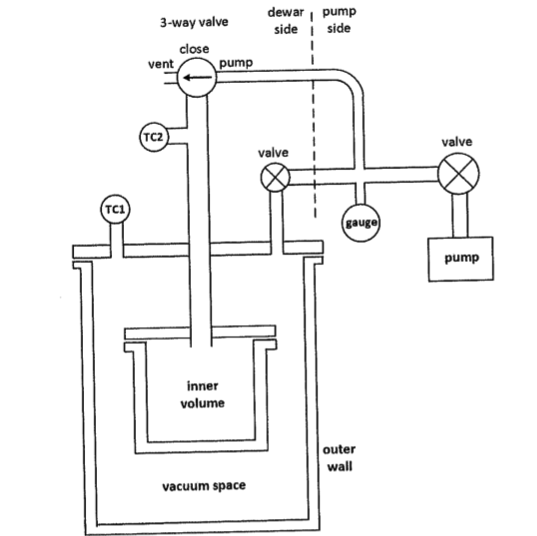
\includegraphics{cryostat_schematic}
  \caption{\label{fig:cryostat} Schematic of cryostat system.}
\end{figure}

\subsubsection{Parts}
The aperatus can be broken down into two main sections (see figure
\ref{fig:cryostat}. The vaccuum pump and the
cryostat. The vacuum pump is a combination of two different systems. The main
pump, and a turbomoleculor pump. See figure \ref{fig:parts} for a diagram of the
parts listed below.

\begin{tabular}{m{4cm}|m{10cm}}
  \hline
  part name & description \\
  \hline
  3-way valve & 
  This controls gas access of the inner can (when installed). The direction of
  the arrow signifies what has access to the inner space. 

  \textbf{left $\rightarrow$ right:} inner can is connected to the vacuum pump.

  \textbf{pointing up:} inner space is held at atmospheric pressure.

  \textbf{right $\rightarrow$ left:} inner space can be filled with some gas connected to the
      nipple of the valve. 

  Note: Once the system contains LN2 this valve can not be changed.\\ 
  \hline
  fill tubes & Gives access to the LN2 resevoir. 1 of 2 tubes must always be
  unobstructed. \\
  \hline
  overpressure valve & Releases gas if pressure in the system is too high.\\
  \hline
  coolant resevoir & 2 litre container for LN2. \\
  \hline
  top of tree & if inner can is present, and the 3-way valve is turned upwards
  this port gives you acess to the inner space. \\
  \hline
\end{tabular}

\vspace{2em}
Not shown in figure \ref{fig:parts} are the 3 vacuum tight connectors which
provide elecrical access to the dewer.

There is a 4-pair connection, 5 pair connection, and 6-pair connection. The 4
pair connection connects the transdiode on the LN2 resevoir to the cryostat box.
The voltage drop across the transdiode is temperature dependent, and is powered
by a \SI{10}{\uA} forward DC current. The other connections here can be ignored for this
experiment. The 5-pair connection is for controll of the heating system. Connect
a D-sub cable from the port connected to these wires to the back of the PI
temperature controller module. This will allow you to control one the FET-based
heating system (see chapter 4 of the official manual for more details). The
series resistor heating system is powered by a current that you apply to 2 of
the banana jack plugs in the cryostat box. These are the only two wires from the
5-pair interface that connect to the banana jack section. The 6-pair plug
corresponds to the screw terminals on the basplate inside the dewer. It is your
job to find a way to organize these electrical connections to get you
measurements. 

\begin{figure}
  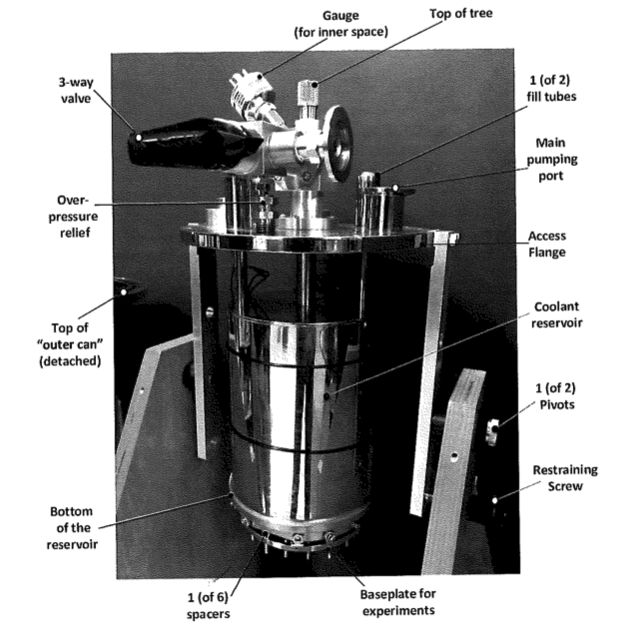
\includegraphics{parts}
  \caption{\label{fig:parts} Photograph of the main parts of the cryostat dewer
  labeled.}
\end{figure}
\subsubsection{Temperature Control and Measurements}
See chapter 4 and 5 of the cryostat manual for details. 

\subsubsection{Operation}
\begin{enumerate}
  \item Assuming the dewer is at standard temperature and pressure, unlatch the
    kf flanges connecting the dewer to the vacuum pump. (There are two both
    connected to the acess flange on the top side of the dewer. Next invert the
    aperatus such that the acess flange is towards the ground and hold the
    system in placing using the large know on the side of the wooden dewer
    holder. Next, unscrew the 4 screws attaching the outer casing to the
    cryostat and remove it. Ensure that you place the outer casing face up to
    not damage the conductive ring around its open side. 

    If you see a silver can (the inner can) on top of the sample plate remove
    it. This is done by unscewing the brass bolts in a star pattern. Remove the
    inner can, being careful not to lose any bolts are washers. 

    (if requred) With the inner can removed connect the sample to the
    nickle-plated baseplate using the screws providied. This is where you test
    all electronic connections to ensure that the system is working correctly
    (or that you know how to make measurements). Each wire can be connected to
    one of the numbered screw panels on the baseplate. Through the 12 wire (or
    6-pair) connection on the acess flange this provides electrical connections
    to the outside world. The terminals marked with numbers are electrically
    connected andd can be ignored for this experiment. 

  \item Depeding on where you would like to keep the sample at vacuum (no inner
    can) or ambient pressure. Rescrew the brass bolts onto the sample plate. If
    you want the sample in the same vacuum as the main system simply screw on 6
    bolts on to the screws attached to the spacers. Use a star pattern and
    follow these methods:
    \begin{enumerate}
      \item all the washers are curved place washes such that one is concave up
	and the other concave down as in figure \ref{fig:washer},
      \item first tighted all the screws with your fingers,
      \item use the allen driver to tighten the brass studs as much as you can with
	one hand,
      \item wait 5 minutes then use the allen driver again to tighten each stud
	as much as you can with one hand.
    \end{enumerate}
    If an inner can is used this must be done for all 18 brass studs.

  \item Connect the KF flanges removed in the first step and turn on the vacuum
    pump. Use the up and down arrows to find the pressure read by the pressure
    gauge in between the vacuum and cryostat. You should see the starting
    pressure is above $10^3$ hPa. The pressure should quickly drop to below
    $10^{-1}$ hPa and within 30 minutes be near $10^{-5}$ hPa. If this does not
    happen and the system is stuck at a high pressure there is a leak in your
    system that you should look for and fix. Ensure the pump is turned off
    before you do this. 

  \item Once the expected pressure is reached it is now time to add the LN2. Use
    the funnel provided to pout the LN2 into the revoir. Ensure that one of the
    fill tubes in unobstructed to allow vapor to escape from the system. A
    funnel at a time begin to cool down the system. It is best to wait a few
    minutes after every 2 funnels worth of fluid is added to the resevoir. It
    should take about 45 minutes for the system to cool to the desired
    temperatures. 

  \item At this point you are ready to take your measurements.

  \item \textbf{Turning off the system} to turn off the system and revert it to
    the warm and dry state we started with close the angular valve directly
    on top of the vacuum pump. Next turn off the vacuum pump (flip the power
    switch) and turn off any heaters. The system will slowly warm up overnight
    and the next morning it should be cool. At this point you can evacuate the
    gas in the inner can, then open the angular valve above the dewer itself.
    This will allow the system to slowly reach atmospheric pressure. After a few
    minutes of waiting the system is again ready to be used. 
\end{enumerate}
\begin{figure}
  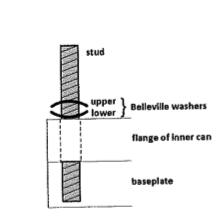
\includegraphics[width=0.5\textwidth]{washer}
  \caption{\label{fig:washer} Sketch of the washer concave up and down.}
\end{figure}
\end{document}
